\documentclass[es]{SurferDesc}%%%%%%%%%%%%%%%%%%%%%%%%%%%%%%%%%%%%%%%%%%%%%%%%%%%%%%%%%%%%%%%%%%%%%%%
%
% The document starts here:
%
\begin{document}
\footnotesize
% Einfache Singularitten 
%
\begin{surferPage}
  \begin{surferTitle}Una Séptica con $99$ Singularidades\end{surferTitle} \\
  % 
  \begin{surferText}
    El número de puntos singulares de una superficie de grado $7$ (séptica)
    no puede ser mayor a 104 (Varchenco).
    La que descubrió Oliver Labs en 2004 tiene $99$, por lo tanto, es posible 
    que existan sépticas con más singularidades. Sin embargo, por el momento
    no se encontró ninguna que supere este récord.
    
    La séptica de Labs tiene la simetría de un heptágono:  
    
    \vspace*{-0.3em}
    \begin{center}
      \begin{tabular}{c@{\qquad}c}
        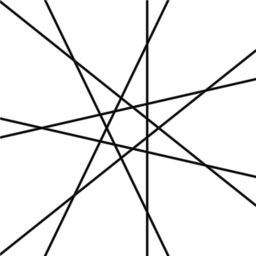
\includegraphics[height=1.5cm]{seven_gon}
        &
        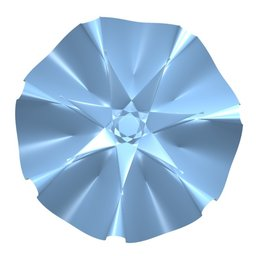
\includegraphics[height=1.5cm]{labs_septic_von_oben}
      \end{tabular}
    \end{center}
    \vspace*{-0.3em}
    Para construir esta superficie, Labs usó el sistema 
    {\sc Singular} (Universidad de Kaiserslautern), un programa especialmente adaptado
    para cálculos de geometría algebraica y singularidades. 
    Además, usó aritmética modular, algo que utilizamos habitualmente cuando hacemos cuentas con las horas:\\
    24:00$=$0:00 y 24:00 $+$ 1:00 hora no es 25:00, sino 1:00.\\
    La aritmética modular funciona de la misma manera, pero usando un número cualquiera
    (el módulo) en lugar de 24.
    En geometría algebraica suele convenir escoger números primos como módulos.
 
%    Eine verwandte Technik kann man auch in der Kryptologie benutzen,
%    um Zahlen in Primfaktoren zu zerlegen.
  \end{surferText}
\end{surferPage}

%%% Local Variables: 
%%% mode: latex
%%% TeX-master: "jDM08_expl_engl"
%%% End: 





\end{document}
%
% end of the document.
%
%%%%%%%%%%%%%%%%%%%%%%%%%%%%%%%%%%%%%%%%%%%%%%%%%%%%%%%%%%%%%%%%%%%%%%%
